% Source: Lecture15.pdf, pages 1-4 (page 5 is blank).
% Title on the source: "Lecture 15 - Renormalization Group, continued".
\lecture{15}
\subsection{Couplings, operators and RG flows}

Let us write a general form for
\begin{equation}
  -\beta\Ham = \sum_iK_i\mathcal{O}_i,
\end{equation}
where the $K_i$ are interaction couplings and the $\mathcal{O}_i$ are operators, e.g.
\begin{equation}
  -\beta\Ham = \sum_{\mathbf r,\,nn(\mathbf r)}K_{nn}\sigma_{\mathbf r}\sigma_{nn(\mathbf r)}
             + \sum_{\mathbf r,\,nnn(\mathbf r)}K_{nnn}\sigma_{\mathbf r}\sigma_{nnn(\mathbf r)} + \cdots,
\end{equation}
with nearest-neighbor and next-nearest-neighbor couplings. Under the real-space RG transformation with
a blocking factor $b$,
\begin{equation}
  K_i' = R_{ib}(\{K_i\}).
\end{equation}
Denote the value of $\{K_i\}$ at a fixed point of the RG as $\{K_i^*\}$. (This is standard notation;
don't confuse it with complex conjugation.) Usually (with some exceptions, e.g.\ in 1D) the RG
transformation will generate additional operators.

\paragraph{Definition.} An operator $\mathcal{O}_i$ is \emph{relevant}, and the corresponding coupling
$K_i$ is relevant, if it must be tuned to a particular value at the critical point and its presence
affects the critical behavior. The opposite is an \emph{irrelevant} operator and the associated coupling.

The iteration of the RG transformation produces a ``flow'' in the space of couplings $\{K_i\}$. One often
approximates this as a continuous flow, although it is really discrete. An illustrative RG flow in the
space of 2 couplings, $K_{nn}$, $K_{nnn}$ (for FM signs $J_{nn}>0$, $J_{nnn}>0$ and $H = 0$):

\begin{diagram}
\begin{tikzpicture}[scale=0.9,>=Stealth]
  \draw (0,0) rectangle (4.5,4);
  \coordinate (fp) at (2,1.8);
  \draw[thick] (0,0) -- (4.5,4);
  \draw[->,thick] (fp) -- (1.0,0.89); \draw[->,thick] (fp) -- (3.2,2.87);
  \draw[->,thick] (0.6,3.2) .. controls (1.4,2.4) .. (1.85,1.95);
  \draw[->,thick] (3.6,0.5) .. controls (2.7,1.3) .. (2.15,1.65);
  \draw[->] (0.6,3.4) .. controls (1.8,2.6) and (2.2,2.6) .. (2.6,3.4);
  \draw[->] (3.7,0.8) .. controls (2.8,1.4) and (2.8,1.0) .. (3.2,0.3);
  \draw[->] (0.4,2.9) .. controls (1.4,2.1) and (1.2,1.4) .. (0.4,1.4);
  \draw[->] (3.9,0.9) .. controls (2.9,1.6) and (3.2,2.2) .. (4.0,2.5);
  \fill[red] (fp) circle (0.08);
  \fill[blue] (0,0) circle (0.08); \fill[blue] (4.5,4) circle (0.08);
  \node[below] at (0,0) {$0$}; \node[below] at (4.5,0) {$\infty$}; \node[below=10pt] at (2.25,0) {$K_{nn}$};
  \node[left] at (0,0) {$0$}; \node[left] at (0,4) {$\infty$}; \node[left=8pt] at (0,2) {$K_{nnn}$};
\end{tikzpicture}
\diagramcaption{An illustrative RG flow. The red point is the critical RG fixed point (RGFP); the blue
points are the $T = \infty$ and $T = 0$ fixed points.}\label{fig:rgflow}
\end{diagram}

The red point is the RG fixed point, RGFP. The flows away from this RGFP are relevant directions, while
the flows toward the RGFP are irrelevant directions. The ``critical curve'' is the curve with the
property that if the system is on this curve, then it stays on the curve, and moves steadily in toward the
RGFP at $(K_{nn}^*,K_{nnn}^*)$ under iterated RG transformations. A relevant perturbation eventually takes
the system away from the critical RGFP to another RGFP. Here there are 2 other RGFPs (blue): (i)
$K_{nn} = K_{nnn} = 0$, the $T = \infty$ RGFP, and (ii) $K_{nn} = K_{nnn} = \infty$, the $T = 0$ RGFP,
where all spins are aligned.

The picture shows a 2-dimensional slice through the space of $\{K_i\}$. This space is formally
infinite-dimensional, since there are an $\infty$ number of irrelevant operators $\mathcal O_i$ that one
can add without changing the critical behavior. (We illustrated this before with, e.g.,
$\sum\sigma_{\mathbf r}\sigma_{\mathbf r+2\hat{\mathbf e}_i}$,
$\sum\sigma_{\mathbf r}\sigma_{\mathbf r+3\hat{\mathbf e}_i}$, \ldots) Thus, the term ``critical surface''
or ``critical submanifold'' is often used synonymously with ``critical curve''.

For a bicritical point in a magnetic system, relevant perturbations include temperature and magnetic field,
since these must both be tuned to specific values $T = T_c$ and $H = H_c = 0$ to get critical behavior. The
presence of $H\ne 0$ explicitly violates the $\mathbb{Z}_2$ or $O(N)$ symmetry. Similarly, adding a term
like a 3-spin coupling to an Ising model, thus violating the $\mathbb{Z}_2$ symmetry, is another relevant
perturbation.

\subsection{Linearized RG near the critical fixed point}

To relate the RG transformations to the critical exponents, one considers the RG transformation in the
local vicinity of the critical point. Take $H = 0$, as before. One linearizes the RG transformation and
diagonalizes the associated RG matrix to obtain the eigenvectors and eigenvalues. Consider 2 couplings to
show how this works. Denote these generically as $K_1$ and $K_2$. The critical RGFP is denoted
$(K_1^*,K_2^*)$. Under an RG transformation,
\begin{equation}
  K_1' = R_1(K_1,K_2),\qquad K_2' = R_2(K_1,K_2).
\end{equation}
Now consider the behavior under the RG transformation near to $(K_1^*,K_2^*)$:
\begin{equation}
  K_1' = R_1(K_1^*+\delta K_1,K_2^*+\delta K_2);
\end{equation}
Taylor-expand this:
\begin{equation}
  K_1' = K_1^* + \left(\pder{R_1}{K_1}\right)_*\delta K_1 + \left(\pder{R_1}{K_2}\right)_*\delta K_2,
\end{equation}
where $*$ means evaluated at the critical RGFP, so $\delta K_1'\equiv K_1'-K_1^*$ is
\begin{equation}
  \delta K_1' = \left(\pder{R_1}{K_1}\right)_*\delta K_1 + \left(\pder{R_1}{K_2}\right)_*\delta K_2 .
\end{equation}
Similarly,
$\delta K_2' = \left(\pder{R_2}{K_1}\right)_*\delta K_1 + \left(\pder{R_2}{K_2}\right)_*\delta K_2$; as a
matrix equation:
\begin{equation}
  \begin{pmatrix}\delta K_1'\\ \delta K_2'\end{pmatrix}
  = \underbrace{\begin{pmatrix}\pder{R_1}{K_1} & \pder{R_1}{K_2}\\[4pt] \pder{R_2}{K_1} & \pder{R_2}{K_2}\end{pmatrix}_*}_{\text{matrix } M}
    \begin{pmatrix}\delta K_1\\ \delta K_2\end{pmatrix}.
\end{equation}
The diagonalization of $M$ yields the eigenvectors $\hat{\mathbf e}_1$, $\hat{\mathbf e}_2$ = directions of
flow into or out from the critical RGFP (as in Figure~\ref{fig:rgflow}, with $K_1$, $K_2$ on the axes).

The eigenvectors and eigenvalues: $M\hat{\mathbf e}_i = \lambda_i\hat{\mathbf e}_i$. Write
\begin{equation}
  \lambda_i = b^{y_i},
\end{equation}
where $b$ = blocking parameter.
\begin{itemize}
  \item $\lambda_i>1\Leftrightarrow y_i>0$: $K_i$ is a relevant parameter, since the RG transformation
    moves the system away from the critical RGFP (indicated as $\hat{\mathbf e}_1$ in the picture).
  \item $\lambda_i<1\Leftrightarrow y_i<0$: $K_i$ is an irrelevant parameter, since the RG transformation
    moves the system toward the critical RGFP ($\hat{\mathbf e}_2$ in the picture).
  \item $\lambda_i = 1\Leftrightarrow y_i = 0$: $K_i$ is a ``marginal'' parameter and a full RG treatment
    requires a higher-order analysis of the behavior near the RGFP.
\end{itemize}
Recall that with $\lambda = L^d$, $\lambda^{a_\tau} = (L^d)^{y_\tau/d} = L^{y_\tau}$, etc. N.B.:
$\hat{\mathbf e}_1$ is not $\perp\hat{\mathbf e}_2$ in general, since $M^T\ne M$; $M$ is not, in general,
symmetric.

The meaning of universality of critical behavior: the details of the flow at points distant from the
critical RGFP depend on the specific form of the RG transformation (block-spin construction) and are not
universal, but the critical behavior, as described by the critical exponents $\{y_i\}$, is universal. Note
that the location of the critical point is not universal and depends on the lattice. For example, for the
isotropic FM Ising model on 2D lattices, with $z = e^{-2K}$,
\begin{equation}
  \text{sq: } z_c = \sqrt2-1 = 0.414,\qquad
  \text{tri: } z_c = \frac{1}{\sqrt3} = 0.577,\qquad
  \text{hc: } z_c = 2-\sqrt3 = 0.268,
\end{equation}
but these all have the same critical behavior. (Recall from the previous lecture that $y_\tau = 1$ and
$y_h = \frac{15}{8}$; $\beta\delta = \frac{y_h}{y_\tau} = \frac18\cdot 15$.) After a blocking
transformation, $\xi' = \xi/b$.

The ``basin of attraction'' of a given RGFP is the subspace in the space of couplings $\{K_i\}$ such that
under RG transformations, a point in this subspace will flow to the RGFP. For the critical RGFP, this is
the critical surface. Further reading: e.g.\ Plischke and Bergersen, chs.~6 and 7 in the 3rd ed.\ (chs.~5
and 6 in the 2nd ed.).

\subsection{A simple explicit RG calculation: the 1D Ising model}

Simple explicit RG calculation: the 1D Ising model with zero external magnetic field, $H = 0$. Without loss
of generality, use the FM sign of coupling, $J>0$, so $K\ge 0$. The spin--spin correlation function is
$\ev{\sigma_0\sigma_r} = v^r$, where $v = \tanh K$. Block-spin transformation, say $b = 2$: the length $r$ on
the original lattice $\to r' = r/b$ on the blocked lattice.

\begin{diagram}
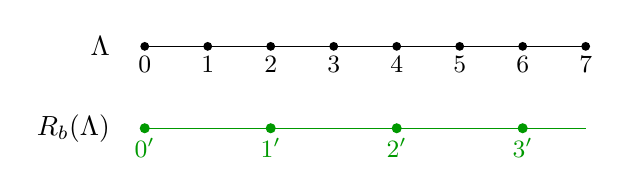
\begin{tikzpicture}[scale=0.8]
  \draw (0,0) -- (7,0); \foreach \x in {0,...,7} {\fill (\x,0) circle (0.07); \node[below,font=\small] at (\x,0) {$\x$};}
  \node[left] at (-0.4,0) {$\Lambda$};
  \begin{scope}[yshift=-1.3cm]
  \draw[green!60!black] (0,0) -- (7,0);
  \foreach \x/\l in {0/0',2/1',4/2',6/3'} {\fill[green!60!black] (\x,0) circle (0.08); \node[below,green!60!black,font=\small] at (\x,0) {$\l$};}
  \node[left] at (-0.4,0) {$R_b(\Lambda)$};
  \end{scope}
\end{tikzpicture}
\diagramcaption{Blocking the 1D lattice with $b = 2$.}
\end{diagram}

On the blocked lattice
\begin{equation}
  \ev{\sigma_{0'}'\sigma_{r'}'} = (v')^{r'},\qquad
  \ev{\sigma_{0'}'\sigma_{1'}'} = \tanh K' = (\tanh K)^2,
\end{equation}
i.e.\ $v' = v^2$:
\begin{equation}
  \tanh K' = (\tanh K)^2,\qquad K' = \operatorname{arctanh}(\tanh K') = \operatorname{arctanh}\left((\tanh K)^2\right).
\end{equation}
Because $\tanh K<1$ for all finite temperatures, $K'<K$, so the RG flow is away from the critical RGFP at
$K = \infty$, i.e.\ $T = 0$, and toward the infinite-temperature RGFP at $K = 0$, $T = \infty$.
Correspondingly the correlation length decreases under the RG flow; $\xi\to\xi/b$.

\begin{diagram}
\begin{tikzpicture}[scale=0.9,>=Stealth]
  \draw (0,0) -- (5,0);
  \foreach \x in {1,2,3,4} \draw[->] (\x+0.3,0) -- (\x,0);
  \fill[blue] (0,0) circle (0.08); \fill[red] (5,0) circle (0.08);
  \node[below,align=center,font=\small] at (0,-0.1) {$K = 0$\\ $T = \infty$};
  \node[below,align=center,font=\small] at (5,-0.1) {$K = \infty$\\ $T = 0$};
  \node[below,font=\small] at (2.5,-0.1) {$K$};
\end{tikzpicture}
\diagramcaption{RG flow of the zero-field 1D Ising model.}
\end{diagram}

Solve for $K'$, using $\operatorname{arctanh}x = \frac12\ln\left(\frac{1+x}{1-x}\right)$:
\begin{equation}
  K' = \frac12\ln\left(\frac{1+v^2}{1-v^2}\right)
     = \frac12\ln\left[\frac{1+\left(\frac{e^K-e^{-K}}{e^K+e^{-K}}\right)^2}{1-\left(\frac{e^K-e^{-K}}{e^K+e^{-K}}\right)^2}\right]
     = \frac12\ln\left[\frac{(e^K+e^{-K})^2+(e^K-e^{-K})^2}{(e^K+e^{-K})^2-(e^K-e^{-K})^2}\right],
\end{equation}
where the numerator is $2(e^{2K}+e^{-2K})$ and the denominator is 4, so
\begin{equation}
  \boxed{K' = \tfrac12\ln\left(\cosh(2K)\right)}.
\end{equation}
So for the zero-field 1D Ising model, there is one relevant parameter, $K$, and the RG flow is from
$K = \infty$ ($T = 0$) to $K = 0$ ($T = \infty$). This is understandable, since under this flow the
correlation length $\xi$ decreases: $\xi\to\xi/b$ (from $\xi = \infty$ at $K = \infty$ to $\xi = 0$ at
$K = 0$). With $\ev{\sigma_0\sigma_r} = v^r = e^{-r/\xi}$,
\begin{equation}
  v = e^{-1/\xi},\qquad \ln v = -\frac1\xi,\qquad
  \xi = -\frac{1}{\ln v} = \frac{1}{\ln\left(\frac{1}{\tanh K}\right)}.
\end{equation}
A special property of this 1D example is that there is only an RG flow away from the critical RGFP. In a
higher-dimensional case, one also generically has an RG flow toward the critical RGFP, as shown in the
previous graph (Figure~\ref{fig:rgflow}).
